\boxde
\BTTN
\Opensolutionfile{ans}[ans/2D1-4-DEON-2]
\begin{ex}%[2D1B4-1]
    Cho hàm số $y=f(x)$ có bảng biến thiên như hình bên. Tổng số tiệm cận đứng và tiệm cận ngang của đồ thị hàm số đã cho là
    \begin{center}
        
\begin{tikzpicture}
            \tkzTabInit[nocadre=false,lgt=1.5,espcl=3,deltacl=0.6]
            {$x$ /0.6,$y’$ /0.6,$y$ /2}
            {$-\infty$ ,$0$, $1$, $+\infty$}
            \tkzTabLine{,-,d,+,0,-,}
            \tkzTabVar{+/$+\infty$,-D-/$-1$/$-\infty$,+/$2$,-/$-\infty$}
        \end{tikzpicture}
    \end{center}
    \choice
    {\True $1$}
    {$3$}
    {$2$}
    {$4$}
    \loigiai{
        Dựa vào bảng biến thiên ta thấy đồ thị hàm số có một tiệm cận đứng $x=0$.
    }
\end{ex}
%62
%63
\begin{ex}%[2D1B4-1]
    Cho hàm số $y=f(x)$ xác định, liên tục trên $\mathbb{R} \backslash \{0;1\}$ và có bảng biến thiên như hình bên. Đồ thị hàm số $y=f(x)$ có
    \begin{center}
        
\begin{tikzpicture}
            \tkzTabInit[nocadre=false,lgt=1.5,espcl=3,deltacl=0.6]
            {$x$ /0.6,$y’$ /0.6,$y$ /2}
            {$-\infty$ ,$0$, $1$, $+\infty$}
            \tkzTabLine{,+,d,+,d,+,}
            \tkzTabVar{-/$-5$,+D-/$+\infty$/$-\infty$,+D-/$3$/$-\infty$,+/$+\infty$}
        \end{tikzpicture}
    \end{center}
    \choice
    {\True $2$ tiệm cận đứng và $1$ tiệm cận ngang}
    {$2$ tiệm cận đứng và $2$ tiệm cận ngang}
    {$1$ tiệm cận đứng và $1$ tiệm cận ngang}
    {$1$ tiệm cận đứng và $2$ tiệm cận ngang}
    \loigiai{
        Dựa vào bảng biến thiên ta thấy đồ thị hàm số có hai tiệm cận đứng $x=0$ và $x=1$; một tiệm cận ngang $y=-5$.
    }
\end{ex}
%64
\begin{ex}%[2D1B4-1]
    Cho hàm số $y=f(x)$ có bảng biến thiên như hình bên. Tổng số tiệm cận đứng và tiệm cận ngang của đồ thị hàm số đã cho là
    \begin{center}
        
\begin{tikzpicture}[scale=0.8]
            \tkzTabInit[nocadre=false,lgt=1.5,espcl=3,deltacl=0.6]
            {$x$ /0.6,$y’$ /0.6,$y$ /2}
            {$-\infty$ ,$-1$, $1$, $+\infty$}
            \tkzTabLine{,+,d,+,0,-,}
            \tkzTabVar{-/$2$,+D-/$4$/$-\infty$,+/$3$,-/$-1$}
        \end{tikzpicture}
    \end{center}
    \choice
    {$1$}
    {\True $3$}
    {$2$}
    {$4$}
    \loigiai{Dựa vào bảng biến thiên ta thấy đồ thị hàm số có một tiệm cận đứng $x=-1$; hai tiệm cận ngang $y=-1$ và $y=2$.
    }
\end{ex}
%65
\begin{ex}%[2D1B4-1]
    Cho hàm số $y=f(x)$ có bảng biến thiên như hình bên. Tổng số tiệm cận đứng và tiệm cận ngang của đồ thị hàm số đã cho là
    \begin{center}
        
\begin{tikzpicture}[scale=0.8]
            \tkzTabInit[nocadre=false,lgt=1.5,espcl=3,deltacl=0.6]
            {$x$ /0.6,$y’$ /0.6,$y$ /2}
            {$-\infty$ ,$0$, $3$, $+\infty$}
            \tkzTabLine{,-,0,+,d,-,}
            \tkzTabVar{+/$8$,-/$1$,+/$4$,-/$2$}
        \end{tikzpicture}
    \end{center}
    \choice
    {$1$}
    {$3$}
    {\True $2$}
    {$4$}
    \loigiai{
        Dựa vào bảng biến thiên ta thấy đồ thị hàm số có hai tiệm cận ngang $y=2$ và $y=8$.
    }
\end{ex}
\begin{ex}%[Nguyễn Văn Sang, dự án Tex hoá đề cương trường Marie Curie - Lần 6]%[2D1Y4-1]
    Đường thẳng nào dưới đây là tiệm cận đứng của đồ thị hàm số $y=\dfrac{2 x+1}{x+1}$?
    \choice
    {$x=1$}
    {$y=-1$}
    {$y=2$}
    {\True $x=-1$}
    \loigiai{
        Tập xác định $\mathscr{D}=\mathbb{R}\setminus\left\lbrace -1\right\rbrace$.
        \begin{itemize}
            \item $\lim\limits_{x \to \pm\infty} y=\lim\limits_{x \to \pm\infty} \dfrac{2x+1}{x+1}=2$ suy ra $y=2$ là tiệm cận ngang.
            \item $\heva{& \lim\limits_{x \to -1^+} \dfrac{2x+1}{x+1}=-\infty \\ & \lim\limits_{x \to -1^-} \dfrac{2x+1}{x+1}=+\infty}$ suy ra $x=-1$ là tiệm cận đứng.
        \end{itemize}
    }
\end{ex}
\begin{ex}%[2D1Y4-1]
    Đồ thị hàm số $y=\dfrac{2x-3}{2x+1}$ có tâm đối xứng là điểm
    \choice
    {\True $M\left(-\dfrac{1}{2};1\right)$}
    {$P\left(-\dfrac{1}{2};2\right)$}
    {$Q\left(-\dfrac{1}{2};-3\right)$}
    {$N\left(1;-\dfrac{1}{2}\right)$}
    \loigiai{
        Tiệm cận đứng, tiệm cận ngang của đồ thị hàm số lần lượt là $x=-\dfrac{1}{2}$ và $y=3$. Tâm đối xứng là điểm $M\left(-\dfrac{1}{2};1\right)$.
    }
\end{ex}
\begin{ex}%[2D1K4-1]
    Đồ thị hàm số $y=\dfrac{\sqrt{x}}{x+1}-\dfrac{1}{x}$ có tất cả bao nhiêu tiệm cận đứng và ngang?
    \choice
    {$0$}
    {$3$}
    {\True $2$}
    {$1$}
    \loigiai{
        Tập xác định $\mathscr{D}=(0;+\infty)$.
        \begin{itemize}
            \item $\lim\limits_{x\to 0^+} \left(\dfrac{\sqrt{x}}{x+1}-\dfrac{1}{x}\right)=-\infty$.
            \item $\lim\limits_{x\to +\infty}\left(\dfrac{\sqrt{x}}{x+1}-\dfrac{1}{x}\right)=0$.
        \end{itemize}
        Suy ra đồ thị hàm số có tiệm cận đứng $x=0$, tiệm cận ngang $y=0$.
    }
\end{ex}
\begin{ex}%[2D1K4-1]
    Số tiệm cận đứng của đồ thị hàm số $y=\dfrac{x^2-3x-4}{x^2-16}$ là
    \choice
    {$2$}
    {$3$}
    {\True $1$}
    {$0$}
    \loigiai{
        Điều kiện xác định $x \ne \pm 4$.\\
        Với điều kiện xác định trên, ta có $y=\dfrac{x^2-3x-4}{x^2-16}=\dfrac{(x+1)(x-4)}{(x-4)(x+4)}=\dfrac{x+1}{x+4}$.\\
        Tiệm cận đứng của đồ thị hàm số là $x=-4$.
    }
\end{ex}
\begin{ex}%[2D1K4-1]
    Số đường tiệm cận đứng và ngang của đồ thị hàm số $y=\dfrac{x-1}{x^2-x-2}$ là
    \choice
    {\True $3$}
    {$1$}
    {$0$}
    {$2$}
    \loigiai{
        Điều kiện xác định $x \ne -1$, $x \ne 2$.\\
        Với điều kiện xác định trên, ta có $y=\dfrac{x-1}{x^2-x-2}=\dfrac{x-1}{(x+1)(x-2)}$.\\
        Tiệm cận đứng của đồ thị hàm số là $x=-1$, $x=2$, tiệm cận ngang của đồ thị hàm số là $y=0$.
    }
\end{ex}
%81
\begin{ex}%[2D1K4-1]
    Cho hàm số $y=f(x)$ có bảng biến thiên như hình bên. Đồ thị hàm số $y=\dfrac{1}{f^2(x)-2f(x)}$ có bao nhiêu tiệm cận đứng?
    \begin{center}
        
\begin{tikzpicture}[scale=0.8]
            \tkzTabInit[nocadre=false,lgt=1.5,espcl=3,deltacl=0.6]
            {$x$ /0.6,$y’$ /0.6,$y$ /2}
            {$-\infty$ ,$-1$, $2$, $+\infty$}
            \tkzTabLine{,+,d,-,0,+,}
            \tkzTabVar{-/$-\infty$,+/$1$,-/$-2$,+/$+\infty$}
        \end{tikzpicture}
    \end{center}
    \choice
    {\True $4$}
    {$3$}
    {$2$}
    {$6$}
    \loigiai{
        Dựa vào bảng biến thiên suy ra $f^2(x)-2f(x)=0 \Leftrightarrow \heva{&f(x)=0\\&f(x)=2}$, phương trình $f(x)=0$ có $3$ nghiệm phân biệt và phương trình $f(x)=2$ có $1$ nghiệm nên đồ thị hàm số đã cho có $4$ tiệm cận đứng.
    }
\end{ex}
%79
\begin{ex}%[2D1K4-1]
    Cho hàm số $y=f(x)$ có bảng biến thiên như hình bên. Tổng số tiệm cận ngang và tiệm cận đứng của đồ thị hàm số $y=\dfrac{2}{f(x)+3}$ là
    \begin{center}
        
\begin{tikzpicture}[scale=0.8]
            \tkzTabInit[nocadre=false,lgt=1.5,espcl=3,deltacl=0.6]
            {$x$ /0.6,$y’$ /0.6,$y$ /2}
            {$-\infty$ ,$-4$, $6$, $+\infty$}
            \tkzTabLine{,-,0,+,0,-,}
            \tkzTabVar{+/$+\infty$,-/$-2$,+/$5$,-/$-\infty$}
        \end{tikzpicture}
    \end{center}
    \choice
    {$4$}
    {$3$}
    {\True $2$}
    {$1$}
    \loigiai{
        Dựa vào bảng biến thiên suy ra
        \begin{itemize}
            \item 	$\lim \limits_{x \to \pm \infty} f(x)=\pm \infty \Leftrightarrow \lim \limits_{x \to \pm \infty}\dfrac{2}{f(x)+3} =0$ nên đồ thị hàm số đã cho có tiệm cận ngang là $y=0$.
            \item $f(x)+3=0 \Leftrightarrow f(x) =-3$, phương trình này có $1$ nghiệm $x=a>6$ nên đồ thị hàm số đã cho có một tiệm cận đứng.
        \end{itemize}
    }
\end{ex}
\begin{ex}%[2D1K4-1]
    Cho hàm số $y=f(x)$ có bảng biến thiên như hình bên. Đồ thị hàm số $y=\dfrac{x+1}{f(x)-4}$ có bao nhiêu tiệm cận đứng?
    \begin{center}
        
\begin{tikzpicture}[scale=0.8]
            \tkzTabInit[nocadre=false,lgt=1.5,espcl=3,deltacl=0.6]
            {$x$ /0.6,$y’$ /0.6,$y$ /2}
            {$-\infty$ ,$-1$, $2$, $+\infty$}
            \tkzTabLine{,+,0,-,0,+,}
            \tkzTabVar{-/$1$,+/$4$,-/$-5$,+/$+\infty$}
        \end{tikzpicture}
    \end{center}
    \choice
    {$1$}
    {$3$}
    {\True $2$}
    {$4$}
    \loigiai{
        Dựa vào bảng biến thiên suy ra
        $f(x)-4=0 \Leftrightarrow f(x) =4$, phương trình này có $1$ nghiệm khác $-1$ và một nghiệm bội chẵn $x=-1$ nên đồ thị hàm số $y=\dfrac{x+1}{f(x)-4}$ có hai tiệm cận đứng.
    }
\end{ex}
\begin{ex}%[2D1K4-1]
    Cho hàm số $y=f(x)$ có bảng biến thiên như hình bên. Đồ thị hàm số $y=\dfrac{x-5}{f(x)-1}$ có bao nhiêu tiệm cận đứng?
    \begin{center}
        
\begin{tikzpicture}
            \tkzTabInit[espcl=3]{$x$ / 1 , $f’(x)$ / 1, $f(x)$ / 2}
            {$-\infty$, $-1$ , $2$, $+\infty$}%
            \tkzTabLine{,-,0,+,d,-,}%
            \tkzTabVar{+/ $+\infty$, - / $-1$, + / $3$,-/$-\infty$}%
            \tkzTabVal[draw]{3}{4}{0.4}{$5$}{$1$}%
            %\tkzTabVal[draw]{2}{3}{0.4}{$e^2$}{$1$}%
        \end{tikzpicture}
    \end{center}
    \choice
    {$1$}
    {$3$}
    {\True $2$}
    {$4$}
    \loigiai{
        Dựa vào bảng biến thiên suy ra
        $f(x)-1=0 \Leftrightarrow f(x) =1$, phương trình này có $2$ nghiệm phân biệt khác $5$ và một nghiệm $x=5$ nên đồ thị hàm số $y=\dfrac{x-5}{f(x)-1}$ có hai tiệm cận đứng.
    }
\end{ex}
\begin{ex}%[VDC5-NgocDungHo]%[2D1G4-3]%
    \immini
    {
        Cho hàm số $f(x)$ có đồ thị như hình bên. Số đường tiệm cận đứng của đồ thị hàm số $y=\dfrac{(x^2-1)(x^2+x)}{[f(x)]^2-2f(x)-3}$ là
        \choice
        {$4$}
        {$5$}
        {\True $3$}
        {$2$}
    }
    {
        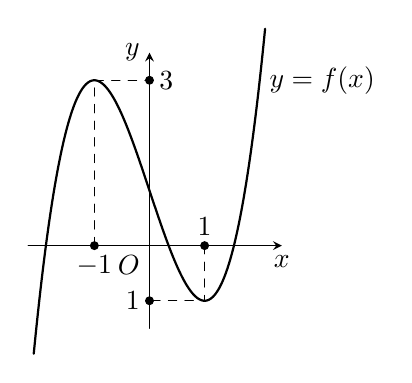
\begin{tikzpicture}[>=stealth,scale=0.7, line join=round, line cap=round]
            \def\f[#1]{(#1)^3-3*(#1)+1)}
            \draw[->] (-2.2,0)--(2.4,0) node [below]{$x$};
            \draw[->] (0,-1.5)--(0,3.5) node [left]{$y$};
            \node at (0,0) [below left]{$O$};
            % \clip;
            \draw[domain=-2.1:2.1,samples=300,thick] plot (\x,{\f[\x]});
            \filldraw (-1,0) node[below]{$-1$} circle (2pt);
            \filldraw (1,0) node[above]{$1$} circle (2pt);
            \filldraw (0,-1) node[ left]{$1$} circle (2pt);
            \filldraw (0,3) node[ right]{$3$} circle (2pt);
            \draw[dashed](-1,0)--(-1,3)--(0,3) (1,0)--(1,-1)--(0,-1);
            \draw (2,3) node[right]{$y=f(x)$};
        \end{tikzpicture}
    }
    \loigiai{
        Xét hàm số $y=g(x)=\dfrac{(x^2-1)(x^2+x)}{[f(x)]^2-2f(x)-3}$.
        \immini
        {
            Giải phương trình $(x^2-1)(x^2+x)=0 \Leftrightarrow \hoac{& x^2-1=0 \\ & x^2+x=0}\Leftrightarrow \hoac{& x=\pm 1 \\ & x=0.}$\\
            Giải phương trình $[f(x)]^2-2f(x)-3=0$\\$ \Leftrightarrow \hoac{& f(x)=-1 \\ & f(x)=3} \Leftrightarrow \hoac{& x = \pm 1 \\ & x=a\\&x=b\;(a<-1<1<b).}$
        }
        {
            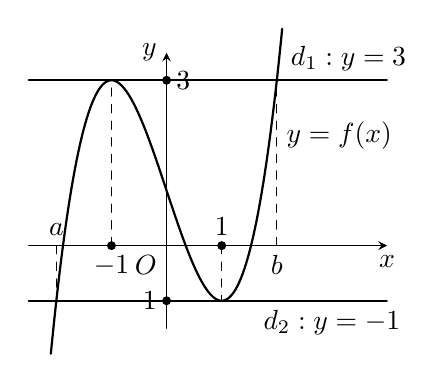
\begin{tikzpicture}[>=stealth,scale=0.7, line join=round, line cap=round]
                \def\f[#1]{(#1)^3-3*(#1)+1)}
                \def\g[#1]{3}
                \def\h[#1]{-1}
                \draw[->] (-2.5,0)--(4,0) node [below]{$x$};
                \draw[->] (0,-1.5)--(0,3.5) node [left]{$y$};
                \node at (0,0) [below left]{$O$};
                % \clip;
                \draw[domain=-2.5:4,samples=300,thick] plot (\x,{\g[\x]});
                \draw[domain=-2.5:4,samples=300,thick] plot (\x,{\h[\x]});
                \draw[domain=-2.1:2.1,samples=300,thick] plot (\x,{\f[\x]});
                \filldraw (-1,0) node[below]{$-1$} circle (2pt);
                \filldraw (1,0) node[above]{$1$} circle (2pt);
                \filldraw (0,-1) node[ left]{$1$} circle (2pt);
                \filldraw (0,3) node[ right]{$3$} circle (2pt);
                \draw[dashed](-1,0)--(-1,3)--(0,3) (1,0)--(1,-1) (2,0)node[below]{$b$}--(2,3) (-2,0)node[above]{$a$}--(-2,-1);
                \draw (2,2) node[right]{$y=f(x)$};
                \draw (3.3,3) node[above]{$d_1:y=3$};
                \draw (3,-1) node[below]{$d_2:y=-1$};
            \end{tikzpicture}
        }
        Trong điều kiện xác định của hàm số $y=g(x)$ ta có thể viết
        $$y=g(x)=\dfrac{x(x-1)(x+1)^2}{(x-a)(x-b)(x-1)^2(x+1)^2}=\dfrac{x}{(x-a)(x-b)(x-1)}$$
        Vậy số tiệm cận đứng của đồ thị hàm số $y=g(x)$ bằng $3$.
    }
\end{ex}
\begin{ex}
    \immini{ %Câu 91.
        Đường cong ở hình bên là đồ thị của hàm số $y = ax^4 + bx^2 +c$. Đồ thị hàm số $g(x) =\dfrac{(x^2-x)\sqrt{x+2}}{(x-2)\cdot f(x+1)}$
        có bao nhiêu đường tiệm cận đứng?
        \choice
        {1}
        {3}
        {4}
        {2}}{
        \begin{tikzpicture}[scale=.8, font=\footnotesize, line join=round, line cap=round, >=stealth]
            \def\xmin{-2}\def\xmax{2}\def\ymin{-3}\def\ymax{1}
            \draw[->] (\xmin-0.2,0)--(\xmax+0.2,0) node[below] {\footnotesize $x$};
            \draw[->] (0,\ymin-0.2)--(0,\ymax+0.2) node[right] {\footnotesize $y$};
            \draw (0,0) node [below left] {\footnotesize $O$};
            \foreach \x in {-1,1}\draw (\x,-0.1)--(\x,0.1) node [above left] {\footnotesize $\x$};
            \foreach \y in {-2}\draw (0.1,\y)--(-0.1,\y) node [ below left] {\footnotesize $\y$};
            \clip (\xmin,\ymin) rectangle (\xmax,\ymax);
            \draw[smooth,samples=200,domain=\xmin:\xmax] plot (\x,{((\x)^4)+((\x)^2)+-2});
        \end{tikzpicture}
    }
    \loigiai{
        * Điều kiện: $\heva{&x \ne 2\\&f(x+1) \ne 0\\&x \ge -2.}$\\
        Nhìn hình vẽ ta thấy
        $f(x+1)=0\Leftrightarrow \hoac{&x+1=-1\\&x+1=1}\Leftrightarrow \hoac{&x=-2&(\text{nghiệm đơn})\\&x=0&(\text{nghiệm đơn}).}$\\
        Vậy $g(x) = \dfrac{(x^2-x)\sqrt{x+2}}{(x-2)\cdot ax^2(x^2+2) }=\dfrac{(x-1)\sqrt{x+2}}{(x-2)\cdot ax(x^2+2)}.$ \\
        Đồ thị hàm số $g(x)$ có 2 đường tiệm cận đứng.}
\end{ex}
\begin{ex}%[Thi thử THPT Yên Phong 1 - Bắc Ninh, 2021]%[Duong Xuan Loi,12EX 6- 2021]%[2D1G4-3]%
    \immini{
        Cho hàm số $y=f(x)$ có đồ thị như hình vẽ. Biết $f'(x)<0$, $\forall x <-1$ và $f'(x)>0$, $\forall x>1$. Khi đó, tổng số tiệm cận của đồ thị hàm số $y=\dfrac{2024}{\sqrt{xf(x+1)}[xf(x+1)+1]-2}$ là
        \choice
        {$1$}
        {$3$}
        {$4$}
        {\True $2$}
    }{
        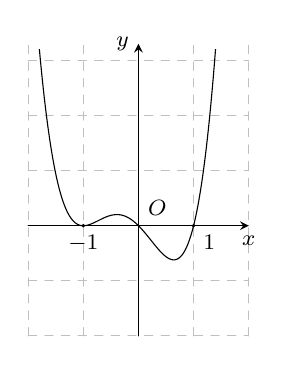
\begin{tikzpicture}[scale=0.7, font=\footnotesize, line join=round, line cap=round,>=stealth]
            \def\xmin{-2} \def\xmax{2}
            \def\ymin{-2} \def\ymax{3.3}
            \draw[color=gray!50,dashed] (\xmin,\ymin) grid (\xmax,\ymax);
            \draw[->] (\xmin,0)--(\xmax,0) node [below]{$x$};
            \draw[->] (0,\ymin)--(0,\ymax) node [left]{$y$};
            \node at (0,0) [above right]{$O$};
            \clip (\xmin+0.1,\ymin+0.1) rectangle (\xmax-0.1,\ymax-0.1);
            \draw[smooth,samples=300,domain=-1.8:1.4] plot(\x,{(\x+1)*(\x+1)*(\x)*(\x-1)});
            \fill (-1,0) circle (1.0pt) node[below]{$-1$} (1,0) circle (1.0pt) node[below right]{$1$};
        \end{tikzpicture}
    }
    \loigiai{
        Xét phương trình $\sqrt{xf(x+1)}[xf(x+1)+1]-2=0.\quad(1)$\\
        Đặt $t=\sqrt{xf(x+1)}(t\geq 0)$, ta được phương trình $t\left(t^2+1\right)=2\Leftrightarrow t^3+t-2=0\Leftrightarrow t=1$.\\
        Với $t=1\Rightarrow\sqrt{xf(x+1)}=1\Leftrightarrow xf(x+1)-1=0$.\\
        Đặt $u=x+1\Rightarrow x=u-1$, ta được phương trình $(u-1)f(u)-1=0\Leftrightarrow f(u)=\dfrac{1}{u-1}.\quad(2)$
        \begin{center}
            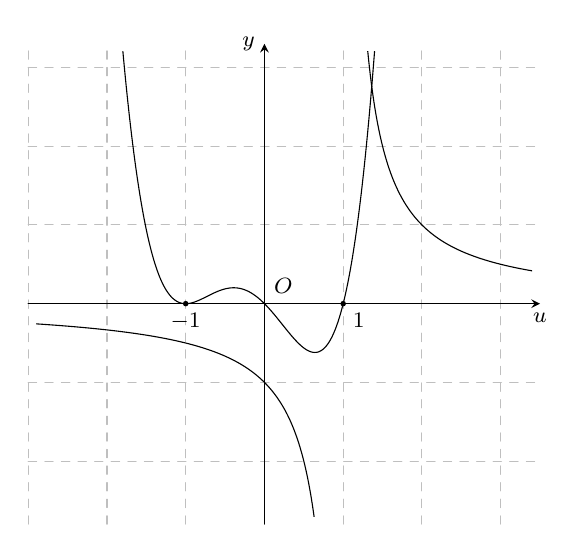
\begin{tikzpicture}[scale=1, font=\footnotesize, line join=round, line cap=round,>=stealth]
                \def\a{0} \def\b{1} \def\c{1} \def\d{-1} % Hệ số
                \def\xmin{-3} \def\xmax{3.5}
                \def\ymin{-2.8} \def\ymax{3.3}
                \draw[color=gray!50,dashed] (\xmin,\ymin) grid (\xmax,\ymax);
                \draw[->] (\xmin,0)--(\xmax,0) node [below]{$u$};
                \draw[->] (0,\ymin)--(0,\ymax) node [left]{$y$};
                \node at (0,0) [above right]{$O$};
                \clip (\xmin+0.1,\ymin+0.1) rectangle (\xmax-0.1,\ymax-0.1);
                \draw[smooth,samples=300,domain=-1.8:1.4] plot(\x,{(\x+1)*(\x+1)*(\x)*(\x-1)});
                \draw[smooth,samples=300,domain=\xmin:(-\d/\c-0.1)] plot(\x,{(\a*(\x)+\b)/(\c*(\x)+\d)});
                \draw[smooth,samples=300,domain=(-\d/\c+0.1:\xmax)] plot(\x,{(\a*(\x)+\b)/(\c*(\x)+\d)});
                \fill (-1,0) circle (1.0pt) node[below]{$-1$} (1,0) circle (1.0pt) node[below right]{$1$};
            \end{tikzpicture}
        \end{center}
        Nhận thấy đồ thị của các hàm số $y=f(u)$, $y=\dfrac{1}{u-1}$ chỉ cắt nhau tại $1$ điểm do đó phương trình $(2)$ có nghiệm duy nhất $\Rightarrow(1)$ có nghiệm duy nhất, suy ra đồ thị có $1$ tiệm cận đứng.\\
        Mặt khác: $\lim\limits_{x\to+\infty} f(x+1)=+\infty\Rightarrow\lim\limits_{x\to+\infty}\dfrac{2021}{\sqrt{xf(x+1)}[xf(x+1)+1]-2}=a>0$.\\
        $\lim\limits_{x\to-\infty} xf(x+1)=-\infty\Rightarrow\lim\limits_{x\to+\infty}\dfrac{2021}{\sqrt{xf(x+1)}[xf(x+1)+1]-2}$ không tồn tại.\\
        Do đó đường thẳng $y=a$ là tiệm cận ngang.}
\end{ex}
\BTTF
\begin{ex}%[EX-TF-2024, Lê Đạt]%[2D1N4-1]
    Cho hàm số $y=f(x)$ có bảng biến thiên như sau
    \begin{center}
        
\begin{tikzpicture}[>=stealth]
            \tkzTabInit[nocadre=false,lgt=1,espcl=3,deltacl=0.6]
            {$x$/.7 ,$y'$/.7,$y$/2}
            {$-\infty$ , $-2$ , $0$, $+\infty$}
            \tkzTabLine{ , - , d , + , d , -, }
            \tkzTabVar{+/$+\infty$ , -D-/$1$/$-\infty$ , +D+/$+\infty$ /$1$, -/$0$}
        \end{tikzpicture}
    \end{center}
    Xét tính đúng sai của các khẳng định sau
    \choiceTF
    {\True $ x=0 $ là tiệm cận đứng của đồ thị hàm số $ y=f(x) $}
    {\True $ x=-2 $ là tiệm cận đứng của đồ thị hàm số $ y=f(x) $}
    {$ x=1 $ là tiệm cận đứng của đồ thị hàm số $ y=f(x) $}
    {\True $ y=0 $ là tiệm cận ngang của đồ thị hàm số $ y=f(x) $}
    \loigiai{
        \begin{itemchoice}
            \itemch $\lim \limits_{x \to 0^-} f(x)=+\infty\Rightarrow x=0$ là đường tiệm cận đứng của đồ thị hàm số $f(x)$.
            \itemch $\lim \limits_{x \to (-2)^+} f(x)=-\infty\Rightarrow x=-2$ là đường tiệm cận đứng của đồ thị hàm số $f(x)$.
            \itemch Đồ thị hàm số chỉ có hai tiệm cận đứng là $ x=0 $ và $ x=-2 $.
            \itemch $\lim \limits_{x \to +\infty} f(x)=0\Rightarrow y=0$ là đường tiệm cận ngang của đồ thị hàm số $f(x)$.
        \end{itemchoice}
    }
\end{ex}
\begin{ex}%[EX-TF-2024, Lê Đạt]%[2D1H4-2]
    Cho hàm số $y=\dfrac{m x^{2}+6 x-2}{x+2}$. Xét tính đúng sai của các khẳng định sau
    \choiceTF
    {Đồ thị hàm số luôn có tiệm cận đứng với mọi $ m $}
    {Đồ thị hàm số không có tiệm cận ngang với mọi $ m $}
    {\True Khi $ m=1 $ đồ thị hàm số có một tiệm cận xiên là $ y=x+4 $ }
    {Đồ thị hàm số luôn có tiệm cận xiên}
    \loigiai{
        \begin{itemchoice}
            \itemch Khi $ m=\dfrac{7}{2} $ hàm số trở thành $y=\dfrac{\dfrac{7}{2} x^{2}+6 x-2}{x+2}=\dfrac{7}{2}\left(x-\dfrac{2}{7} \right) $ suy ra đồ thị hàm số không có tiệm cận đứng.
            \itemch Khi $ m=0 $ hàm số trở thành $ y=\dfrac{6x-2}{x+2} $ từ đó suy ra đồ thị hàm số có $ y=6 $ là tiệm cận ngang.
            \itemch Khi $ m=1 $ hàm số trở thành $ y=\dfrac{x^2+6x-2}{x+2}=x+4-\dfrac{10}{x+2} $ từ đó suy ra $ y=x+4 $ là một tiệm cận ngang.
            \itemch Khi $ m=0 $ hàm số trở thành $ y=\dfrac{6x-2}{x+2} $ từ đó suy ra đồ thị hàm số có $ y=6 $ là tiệm cận ngang, $ x=-2 $ là tiệm cận đứng và không có tiệm cận xiên.
        \end{itemchoice}
    }
\end{ex}
\begin{ex}%[EX-TF-2024, Lê Đạt]%[2D1H4-3]
    \immini{Cho hàm số $y=f(x)$ có đồ thị như hình bên. Xét tính đúng sai của các khẳng định sau
        \choiceTF
        {\True $ x=0 $ là một đường tiệm cận đứng của đồ thị hàm số}
        {$ y=-x $ là một đường tiệm cận xiên của đồ thị hàm số}
        {\True $ y=x $ là một đường tiệm cận xiên của đồ thị hàm số}
        {Đồ thị hàm số có ba đường tiệm cận}
    }{
        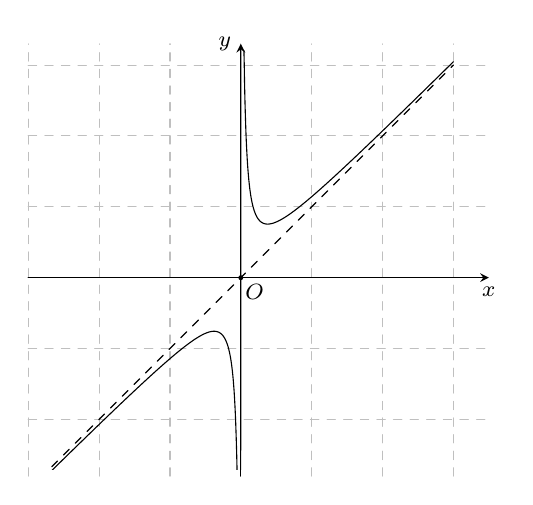
\begin{tikzpicture}[scale=.9, font=\footnotesize, line join=round, line cap=round,>=stealth]
            \def\a{0} \def\b{1} \def\c{1} \def\d{-1} % Hệ số
            \def\xmin{-3} \def\xmax{3.5}
            \def\ymin{-2.8} \def\ymax{3.3}
            \draw[color=gray!50,dashed] (\xmin,\ymin) grid (\xmax,\ymax);
            \draw[->] (\xmin,0)--(\xmax,0) node [below]{$x$};
            \draw[->] (0,\ymin)--(0,\ymax) node [left]{$y$};
            \fill (0,0) circle(1pt) node[shift=(-45:0.25)]{$O$};
            \clip (\xmin+0.1,\ymin+0.1) rectangle (\xmax-0.1,\ymax-0.1);
            \draw[smooth,samples=300,domain=-3:3] plot(\x,{\x+1/(7*\x)});
            \draw[dashed,smooth,samples=300,domain=-3:3] plot(\x,{\x});
            %	\fill (-1,0) circle (1.0pt) node[below]{$-1$} (1,0) circle (1.0pt) node[below right]{$1$};
    \end{tikzpicture}}
    \loigiai{
        \begin{itemchoice}
            \itemch $ x=0 $ là một đường tiệm cận đứng của đồ thị hàm số.
            \itemch	$ y=x $ là một đường tiệm cận xiên của đồ thị hàm số.
            \itemch $ y=x $ là một đường tiệm cận xiên của đồ thị hàm số.
            \itemch Đồ thị hàm số có $ x=0 $ là tiệm cận đứng và $ y=x $ là tiệm cận xiên nên có hai tiệm cận.
        \end{itemchoice}
    }
\end{ex}
\begin{ex}
    \immini
    {
        Cho hàm số $y=f(x)$ có đạo hàm liên tục trên $R$. Hàm số $y=f^{\prime}(x)$ có đồ thị như hình bên. Xác định tính đúng, sai của các mệnh đề sau
        \choiceTF
        {Hàm số $y=f(x)$ có hai cực trị}
        {Hàm số $y=f(x)$ đồng biến trên khoảng $(1 ;+\infty)$}
        {\True $f(1)>f(2)>f(4)$.}
        {\True Trên đoạn $[-1 ; 4]$, giá trị lớn nhất của hàm số $y=f(x)$ là $f(1)$.}
    }
    {
        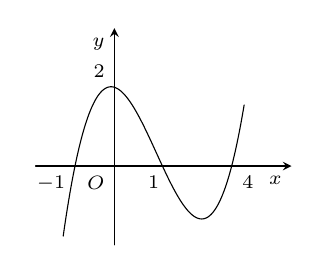
\begin{tikzpicture}[line join=round, line cap=round,>=stealth,font=\scriptsize]
            \begin{scope}[scale=0.5]
                \tikzset{label style/.style={font=\footnotesize}}
                \def \xmin{-2}
                \def \xmax{4.5}
                \def \ymin{-2}
                \def \ymax{3.5}
                \def \hamso{0.55*(\x)^3-1.76*(\x)^2-0.31*(\x)+2}
                \draw[->] (\xmin,0)--(\xmax,0) node[below left] {$x$};
                \draw[->] (0,\ymin)--(0,\ymax) node[below left] {$y$};
                \draw (0,0) node [below left] {$O$};
                \begin{scope}
                    \clip (\xmin+0.01,\ymin+0.01) rectangle (\xmax-0.01,\ymax-0.01);
                    \draw[samples=350,domain=-1.3:3.3,smooth,variable=\x] plot (\x,{\hamso});
                \end{scope}
                \draw (-1,0) node[below left]{$-1$} (1,0) node[below]{$1$} (3,0) node[below right]{$4$} (0,2) node[above left]{$2$};
            \end{scope}
        \end{tikzpicture}
    }
    \loigiai{}
\end{ex}
\begin{ex}
    \immini{Cho hàm số $y=f(x)$ liên tục trên đoạn $\left[0 ; \frac{7}{2}\right]$ có đồ thị hàm số $y=f^{\prime}(x)$ như hình vẽ.
        \choiceTF
        {\True Hàm số $y=f(x)$ đồng biến trên khoảng $\left(3 ; \frac{7}{2}\right)$}
        {\True $f(0)>f(3)$}
        {$f(3)>f\left(\frac{7}{2}\right)$}
        {Hàm số $y=f(x)$ đạt giá trị nhỏ nhất trên đoạn $\left[0 ; \frac{7}{2}\right]$ tại điểm $x_0=\frac{7}{2}$}
    }{\begin{tikzpicture}[>=stealth, samples=100,smooth,y=.7cm,font=\scriptsize]
            \begin{scope}[scale=.7]
                \draw[->] (-1,0)--(4.5,0) node[below] {$x$};
                \draw[->] (0,-2)--(0,4) node[right] {$y$};
                \draw (0,0) node [below left] {$O$};
                \draw[dashed] (3.6,0)--(3.6,4);
                \draw[samples=200,domain=0.2:3.6,smooth,variable=\x]
                plot (\x,{1.06*(\x)^3-5.3*(\x)^2+7.23*(\x)-3});
                \path
                (3.6,0)node[below]{$\dfrac{7}{2}$}
                (3,0)node[above left]{$3$}
                (1,0)node[above]{$1$}
                ;
            \end{scope}
    \end{tikzpicture}}
    \loigiai{}
\end{ex}
\BTTL
\begin{ex}%[2D1K4-2]%
    Đồ thị hàm số $y=\dfrac{(2m+1)x+3}{x+1}$ có đường đường tiệm cận đi qua điểm $A(-2;7)$ khi và chỉ khi
    \shortans{$m=3$}
    %	\choice
    %	{\True $m=3$}
    %	{$m=1$}
    %	{$m=-1$}
    %	{$m=-3$}
    \loigiai{
        Từ đề bài, suy ra $2m+1=7 \Leftrightarrow m=3$.\\
        Suy ra $m+n=0$.
    }
\end{ex}
\begin{ex}%[Học kì 1, THPT Nguyễn Thi Minh Khai - Hà Nội, 2020-2021]%[Bùi Mạnh Tiến, 12EX5]%[2D1K4-2]%
    Cho hàm số $ y=\dfrac{2mx+m}{x-1}$. Với giá trị nào của tham số $m$ thì đường tiệm cận đứng, tiệm cận ngang của đồ thị hàm số cùng hai trục tọa độ tạo thành một hình chữ nhật có diện tích bằng $8$?
    \shortans{$m=\pm 4$}
    %	\choice
    %	{$ m=2$}
    %	{ $m=\pm 2$}
    %	{\True $m=\pm 4$}
    %	{$ m=\pm\dfrac{1}{2}$}
    \loigiai{
        Hàm số $y=\dfrac{2mx+m}{x-1}$ có $a=2m$, $b=m$, $c=1$, $d=-1$.\\
        Tiệm cận ngang $y=\dfrac{a}{c}=2m$.\\
        Tiệm cận đứng $x=-\dfrac{d}{c}=1$.\\
        Diện tích hình chữ nhật tạo thành bởi hai đường tiệm cận và hai trục tọa độ có diện tích
        \begin{align*}
            |2m|\cdot 1=8\Leftrightarrow m=\pm 4.
        \end{align*}
    }
\end{ex}
\begin{ex}%[KSCL lần 1, Liễn Sơn - Vĩnh Phúc, 2021]%[Phạm Doãn Lê Bình, 12EX4-2021]%[2D1K4-2]%
    Cho hàm số $y=\dfrac{x-\sqrt{x^2+2x}}{x^2+mx-m-3}$ có đồ thị $(C)$. Giá trị của $m$ để $(C)$ có đúng hai tiệm cận thuộc tập nào sau đây?
    \shortans{$(-5;2)$}
    %	\choice
    %	{$(-2;1)$}
    %	{$(1;5)$}
    %	{$(5;8)$}
    %	{\True $(-5;2)$}
    \loigiai{
        Điều kiện xác định của hàm số đã cho $\heva{& \hoac{ & x\ge 0 \\ & x\le -2}\\ & x^2+mx-m-3\ne 0.}$\\
        Ta có $\lim \limits_{x\to +\infty} y = \lim \limits_{x\to -\infty} y = 0$ nên $(C)$ có một tiệm cận ngang $y=0$.\\
        Xét phương trình $x^2+mx-m-3=0$.\hfill $(1)$\\
        Ta có
        \begin{itemize}
            \item $\Delta = m^2+4m+12>0$, $\forall m \in \mathbb{R}$.\\ Vậy phương trình $(1)$ luôn có hai nghiệm phân biệt $x_1,x_2$ ($x_1<x_2$).
            \item $x-\sqrt{x^2+2x}=0 \Leftrightarrow \heva{& x\ge 0 \\ & x^2=x^2+2x} \Leftrightarrow x=0$.
            \item Phương trình $(1)$ có nghiệm $x=0 \Leftrightarrow m=-3$. Với $m=-3$ ta có
            $ y =\dfrac{x-\sqrt{x^2+2x}}{x^2-3x}.$
            Khi đó
            \begin{eqnarray*}
                & \lim \limits_{x\to 0^+} y & =\lim \limits_{x\to 0^+} \dfrac{x-\sqrt{x^2+2x}}{x^2-3x}\\
                & & =\lim \limits_{x\to 0^+} \dfrac{-2x}{(x^2-3x)\left( x+\sqrt{x^2+2x}\right)}\\
                & & = \lim \limits_{x\to 0^+} \dfrac{-2}{(x-3)\left( x+\sqrt{x^2+2x}\right)}=+\infty
            \end{eqnarray*}
            và $\lim \limits_{x\to 3^+} y =-\infty$
            nên $(C)$ có thêm hai tiệm cận đứng $x=0$ và $x=3$ (không thỏa yêu cầu bài toán).
            \item Với $m\ne -3$ thì $(C)$ có đúng hai tiệm cận khi và chỉ khi $\hoac{& x_1<-2<x_2<0 &(2)\\ & -2<x_1<0<x_2. & (3)}$
            \item Đặt $f(x)=x^2+mx-m-3$. Ta có
            $(2)\Leftrightarrow \heva{& f(-2)< 0 \\ & f(0) >0 \\ & 0>-m} \Leftrightarrow \heva{& m>\dfrac{1}{3}\\ & m<-3 \\ & m>0}\Leftrightarrow m \in \varnothing.$
            \item $(3)\Leftrightarrow \heva{& f(-2)> 0 \\ & f(0) <0 \\ & -2<-m} \Leftrightarrow \heva{& m<\dfrac{1}{3}\\ & m>-3 \\ & m<2}\Leftrightarrow -3<m<\dfrac{1}{3}.$
        \end{itemize}
        Vậy $m\in \left(-3;\dfrac{1}{3}\right)$.
    }
\end{ex}
\begin{ex}%[kiểm tra GHK1, Sở GD và ĐT - Vĩnh Phúc, 2021]%[Huỳnh Xuân Tín, 12EX4]%[2D1K4-2]%
    Gọi $S$ là tập tất cả các giá trị của tham số $m$ để đồ thị hàm số	$y=\dfrac{x-3}{x^2-2x-m}$ có đúng một đường
    tiệm cận đứng. Tính tổng các phần tử của tập $S$.
    \shortans{$2$}
    %	\choice
    %	{$-1$}
    %	{\True $2$}
    %	{$-6$}
    %	{$1$}
    \loigiai{
        Để đồ thị hàm số	$y=\dfrac{x-3}{x^2-2x-m}$ có đúng một đường
        tiệm cận đứng, ta có hai trường hợp sau
        \begin{enumerate}[TH 1.]
            \item $x^2-2x-m=0$ có nghiệm kép $\Leftrightarrow \Delta'=1+m=0\Leftrightarrow m=-1$.
            \item $x^2-2x-m=0$ có hai nghiệm phân biệt trong đó có một nghiệm bằng $3$
            \[\Leftrightarrow \heva{&\Delta'=1+m>0\\& 3^2-6-m=0}\Leftrightarrow\heva{&m>-1\\&m=3}\Leftrightarrow m=3.\]
        \end{enumerate}
        Khi đó $S=\{-1;3\}$ và có tổng là $2$.
    }
\end{ex}
\begin{ex}
    Tốc độ phản ứng của enzyme theo nồng độ cơ chất \( S \) được mô tả bởi phương trình Michaelis-Menten: $v(S) = \dfrac{V_{\text{max}} S}{K_m + S}$,
    trong đó \( v(S) \) là tốc độ phản ứng, \( S \) là nồng độ cơ chất, \( V_{\text{max}} \) là tốc độ tối đa, và \( K_m \) là hằng số Michaelis. Xác định và nêu ý nghĩa của đường tiệm cận đứng của hàm số này.
    \shortans{không có TCĐ, tốc độ phản ứng không thể tới vô hạn}
    \loigiai{
        Để tìm tiệm cận đứng, ta xét các giá trị của \( S \) làm cho mẫu số của phương trình bằng 0:
        \[
        K_m + S = 0 \Rightarrow S = -K_m
        \]
        Vì nồng độ cơ chất \( S \) không thể âm, không có tiệm cận đứng trong trường hợp này.
        \textbf{Ý nghĩa:} Điều này có nghĩa là tốc độ phản ứng enzyme không có giá trị nào dẫn đến tốc độ phản ứng tiến đến vô hạn trong phạm vi các giá trị hợp lý của \( S \).}
\end{ex}
\begin{ex}
    \immini{Một ống khói của nhà máy điện hạt nhân có mặt cắt là một hypebol $(H)$ có phương trình chính tắc là $\dfrac{x^2}{27^2}-\dfrac{y^2}{40^2}=1$ (Hình $1.25$). Xét hai nhánh bên trên $Ox$ của $(H)$ là đồ thị $(C)$ của hàm số $y=\dfrac{40}{27}\sqrt{x^2-27^2}$ (phần nét liền đậm). Tìm tất cả các đường tiệm cận xiên của $(C)$.}{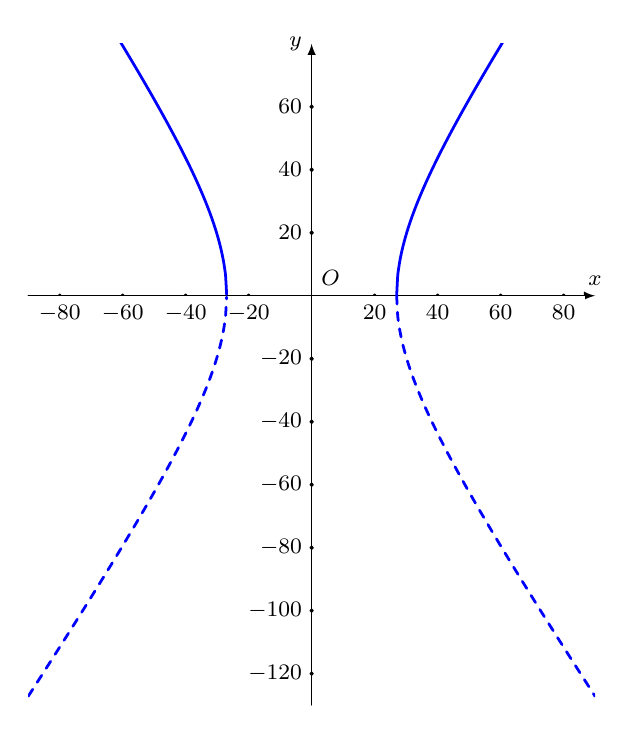
\begin{tikzpicture}[>=latex,line join=round, line cap=round, scale=.04, font=\footnotesize]
            \draw[->] (-90,0)--(90,0) node[above]{$x$};
            \draw[->] (0,-130)--(0,80) node[left]{$y$};
            \foreach \x in {-80,-60,-40,-20,20,40,60,80}
            \draw[fill=black] (\x,0) circle (15pt) node[below, fill=white]{$\x$};
            \foreach \y in {-120,-100,-80,-60,-40,-20,20,40,60}
            \draw[fill=black] (0,\y) circle (15pt) node[left]{$\y$};
            \clip (-90,-130) rectangle (90,80);
            \draw[samples=200,smooth,blue,line width=1] plot[domain=-90:-27] (\x,{40*sqrt((\x)^2-27^2)/27});
            \draw[samples=200,smooth,blue,line width=1] plot[domain=27:90] (\x,{40*sqrt((\x)^2-27^2)/27});
            \draw[samples=200,smooth,blue,line width=1, dashed] plot[domain=-90:-27] (\x,{-40*sqrt((\x)^2-27^2)/27});
            \draw[samples=200,smooth,blue,line width=1, dashed] plot[domain=27:90] (\x,{-40*sqrt((\x)^2-27^2)/27});
            \draw (0,0) node[above right]{$O$};
    \end{tikzpicture}}
    \shortans{$y=\pm \dfrac{40}{27}$}
    \loigiai{
        Ta có
        \allowdisplaybreaks
        \begin{eqnarray*}
            a&=&\lim\limits_{x\to+\infty}\dfrac{f(x)}{x}	 =\lim\limits_{x\to+\infty}\dfrac{\dfrac{40}{27}\sqrt{x^2-27^2}}{x}\\
            &=&\lim\limits_{x\to+\infty}\dfrac{\dfrac{40}{27}x\sqrt{1-\dfrac{27^2}{x^2}}}{x}
            =\lim\limits_{x\to+\infty}\dfrac{40}{27}\sqrt{1-\dfrac{27^2}{x^2}}
            =\dfrac{40}{27}.\\
            b&=&\lim\limits_{x\to+\infty}\left[f(x)-ax\right]
            =\lim\limits_{x\to+\infty}\left[\dfrac{40}{27}\sqrt{x^2-27^2}-\dfrac{40}{27}x\right]\\
            &=&\lim\limits_{x\to+\infty}\dfrac{40}{27}\left(\sqrt{x^2-27^2}-x\right)
            =\lim\limits_{x\to+\infty}\dfrac{40}{27}\cdot\dfrac{x^2-27^2-x^2}{\sqrt{x^2-27^2}+x}\\
            &=&\lim\limits_{x\to+\infty}\dfrac{40}{27}\cdot\dfrac{-27^2}{x\left(\sqrt{1-\dfrac{27}{x^2}}+1\right)}
            =0.
        \end{eqnarray*}
        Vậy đường thẳng $y=\dfrac{40}{27}x$ là một tiệm cận xiên của đồ thị.\\
        Tương tự, $\lim\limits_{x\to-\infty}\dfrac{f(x)}{x}=-\dfrac{40}{27}\Rightarrow a=-\dfrac{40}{27}$; $\lim\limits_{x\to-\infty} \left[f(x)-ax\right]=0\Rightarrow b=0$.\\
        Vậy đường thẳng $y=-\dfrac{40}{27}x$ là tiệm cận xiên của đồ thị.
    }
\end{ex}

\Closesolutionfile{ans}